\documentclass[a4paper, 12pt]{article}
\usepackage{booktabs}
\usepackage{amssymb}
\usepackage{amsmath}
\usepackage{graphicx}
\usepackage{systeme}

\begin{document}

\vspace{0.5cm}
% \noident\textbf{RESUMO.}
% Neste relatório analisaremos o problema de
% transferência de calor em regime permanente em superfícies estendidas 
% unidimensionais. Começamos fazendo uma introdução do problema, em seguida apresentamos a formulação numérica do problema, resultados e conclusão. 

\section{INTRODUÇÃO}


\begin{equation}
  \label{heat}
  \frac{d^2 T}{dx^2} - m^2 [T(x) - T_{amb}] = 0
\end{equation}
sendo o termo $T_{amb}$ é a temperatura ambiente, $T(x)$ é a temperatura ao longo do atleta, $m^2$ é o 

\begin{equation}
  \label{m2}
  m^2 = \frac{hP}{kA}
\end{equation}
onde 
\section{O PROBLEMA}

O problema de transferência de calor é um problema de segunda ordem \ldots
A maneira mais apropriada de resolver o problema analítico descrito em~\ref{heat} é por meio da utilização da técnica da equação característica. Nela escreve-se a equação diferencial de segunda
ordem em uma equação polinomial de segundo grau para resolver o problema homogêneo e após isso, encontra-se a solução particular. Reescreve-se~\label{heat} de maneira a separar todos os termos $T(x)$ do
`resto'.

\begin{equation}
  \label{heatmodified}
  \frac{d^2 T}{dx^2} - m^2 T(x) = - m^2 T_{amb} 
\end{equation}

a equação característica $Z(r)$ é obtida a partir da reformulação da EDO em forma polinomial, e com a obtenção das raízes, gera-se a solução homogênea da EDO 
\begin{equation}
  \label{caracter}
  Z(r) = r^2 - m^2, Z(r) = 0  \rightarrow  r^2 - m^2 = 0 \rightarrow  r^2 = m^2 \rightarrow  r = \pm m 
\end{equation}

a solução homogênea $y_{h}(x)$ é escrita como 
\begin{equation}
  \label{homogenous}
  y_{h}(x) = c_1 \exp(mx) + c_2 \exp(-mx)
\end{equation}


A abordagem numérica utilizada para este trabalho será apoiada na utilização de métodos de diferenças finitas, com ênfase em uma abordagem por diferenças centradas de três pontos para a 
segunda derivada. 
Tal formulação é obtida a partir da discretização do domínio, onde $t_i = T(x_i)$, $t_{i+1} = T(x_i + \Delta x)$, $t_{i-1} = T(x_i - \Delta x)$. 
Fazendo a aproximação em série de Taylor em $u_{i+1}$ e $u_{i-1}$ resulta em 

\begin{equation}
  \label{uip1}
  t_{i+1} = t_i+\sum_{j=1}^n \frac{\Delta x^j}{j!}\frac{d^jT}{dx^j}\Bigm\lvert_{x_i} \\ 
\end{equation}
\begin{equation}
  \label{uim1}
  t_{i-1} = t_i+\sum_{j=1}^n \frac{(-\Delta x)^j}{j!}\frac{d^jT}{dx^j}\Bigm\lvert_{x_i}
\end{equation}

Somando as equações~\ref{uip1} e~\ref{uim1}, os termos ímpares se cancelam resultando em 
\begin{equation}
  \label{uims}
  t_{i+1}+t_{i-1}= 2t_i + \frac{2\Delta x^2}{2}\frac{d^2T}{dx^2}\Bigm\lvert_{x_i} + \frac{2\Delta x^4}{4!}\frac{d^4T}{dx^4}\Bigm\lvert_{x_i} + \ldots
\end{equation}

isolando o termo da derivada segunda, obtém-se

\begin{equation}
  \label{udv2}
  \frac{d^2T}{dx^2}\Bigm\lvert_{x_i}=\frac{t_{i+1}+t_{i-1} - 2t_i}{\Delta x^2} - \Big( \frac{2\Delta x^2}{4!}\frac{d^4T}{dx^4}\Bigm\lvert_{x_i} + \ldots \Big)  
\end{equation}

aplicando \ref{udv2} em \ref{heat} e separando o erro numérico 
\begin{equation}
  \label{udv2n}
  \frac{t_{i+1}+t_{i-1} - 2t_i}{\Delta x^2} - m^2 [t_i - T_{amb}] = \Big( \frac{2\Delta x^2}{4!}\frac{d^4T}{dx^4}\Bigm\lvert_{x_i} + \ldots \Big) 
\end{equation}
que resulta na discretização completa de \ref{heat} que possui ordem $\mathcal(O)(\Delta x^2)$ tendo em vista que este é o maior erro que o método possui. Separando os termos que possuem da deriva dos que não são, implica em
\begin{equation}
  \label{udv2r}
  t_{i+1}+t_{i-1} - 2t_i = m^2 [t_i - T_{amb}] (\Delta x)^2+\mathcal(O)(\Delta x^2)
\end{equation}

considerando as condições de contorno, monta-se um sistema de equações abaixo

\begin{equation}
  \label{syseq}
  \systeme*{t_2 - 2t_1 + t_0= m^2[t_1-T_{amb}](\Delta x)^2, t_3 - 2t_2 + t_1= m^2[t_2-T_{amb}](\Delta x)^2, t_4 - 2t_3 + t_2= m^2[t_3-T_{amb}](\Delta x)^2,t_5 - 2t_4 + t_3= m^2[t_4-T_{amb}](\Delta x)^2, t_6 - 2t_5 + t_4= m^2[t_5-T_{amb}](\Delta x)^2, t_7 - 2t_6 + t_5= m^2[t_6-T_{amb}](\Delta x)^2,t_8 - 2t_7 + t_6= m^2[t_7-T_{amb}](\Delta x)^2,t_9 - 2t_8 + t_7= m^2[t_8-T_{amb}](\Delta x)^2, t_{10} - 2t_9 + t_8= m^2[t_9-T_{amb}](\Delta x)^2}
\end{equation}
com $t_0 = T_0$ e $T_{10} = T_{N}$
% origem na definição de derivada. A derivada é fornecida pela definição de limite 
% 
% \begin{equation}
%   \label{f1}
%   \frac{dF}{dx} = \lim_{\Delta x \to 0} \frac{F(x + \Delta x) - F(x)}{\Delta x}
% \end{equation}
% 
% Seja portato, $G(x) =  \dot{F}(x)$ a derivada de primeira ordem da função genérica $f$, a derivada de segunda de $f$ pode ser escrita como a derivada primeira de $g$, portanto 
% 
% \begin{equation}
%   \label{f2}
%   \frac{d^2 F}{dx^2} = \frac{dG}{dx} = \lim_{\Delta x \to 0} \frac{G(x + \Delta x) - G(x)}{\Delta x}
% \end{equation}
% substituindo a definição de derivada contida em~\ref{f1} na equação~\ref{f2}
% 
% \begin{equation}
%   \label{f2d}
%   \frac{d^2 F}{dx^2} =  \lim_{\Delta x \to 0} \frac{\frac{F(x + \Delta x+ \Delta x)-F(x + \Delta x)}{\Delta x} - \frac{F(x + \Delta x) - F(x)}{\Delta x}}{\Delta x} = \lim_{\Delta x \to 0} \frac{F(x + 2\Delta x) - 2F(x + \Delta x) - F(x)}{\Delta x^2}
% \end{equation}
% Ao discretizar o domínio, $f_i = F(x_i)$, $f_i = F(x_i)$, $f_{i-1} = F(x_i - \Delta x)$, portanto, obtém-se a aproximação avançada no espaço 


\section{RESULTADOS NUMÉRICOS}

Nesta seção apresentamos alguns resultados referêntes ao modelo discutido acima. 
Para este trabalho, foram disponibilizados certas condições para que fosse simulado, mas também mostrando alterações em certos valores e analisamos o que isso representa.
\begin{table}[ht!]
\centering
\begin{tabular}{cc}
  $T_0:$ & $180^\circ$ C \\
  $T_n:$ & $65^\circ$ C  \\
  $T_{amb}:$ & $20^\circ$ C  \\
   h: & $150\frac{W}{m^2K}$ \\
   k: & $120\frac{W}{mK}$ \\
   D: & $3,5 \times 10^{-3}m$ \\
   L: & $0,15m$ \\
\end{tabular}
\end{table}
Abaixo apresenta-se o resultado desta simulação
\begin{figure}[ht!]
\centering
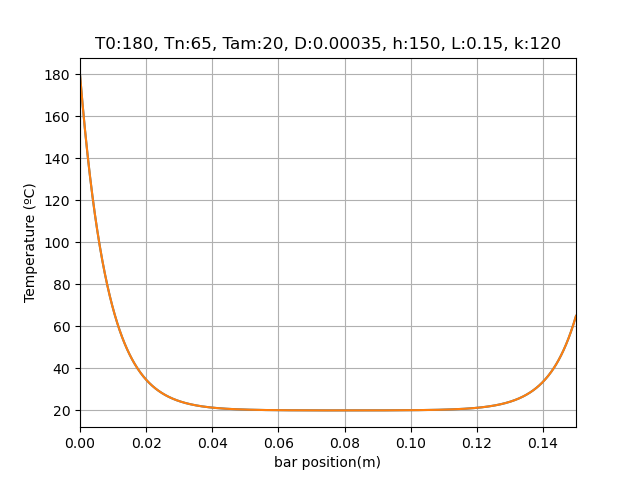
\includegraphics[scale=0.8]{figs/fst.png}
\end{figure}
O próximo experimento foi $m^2 = 0$, que para fins de simplificação, foi feito removendo a troca de calor por convecção($k$). 
\begin{figure}[ht!]
\centering
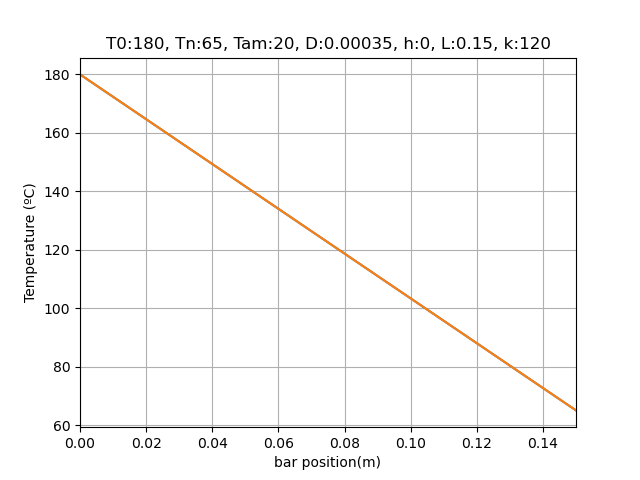
\includegraphics[scale=0.8]{figs/snd.png}
\end{figure}

O próximo experimento foi $m^2$ tendendo com valores muito altos afim de reproduzir $m^2 \to \infty$, que para fins de simplificação, foi feio fazendo $D \to 0$. 
\begin{figure}[ht!]
\centering
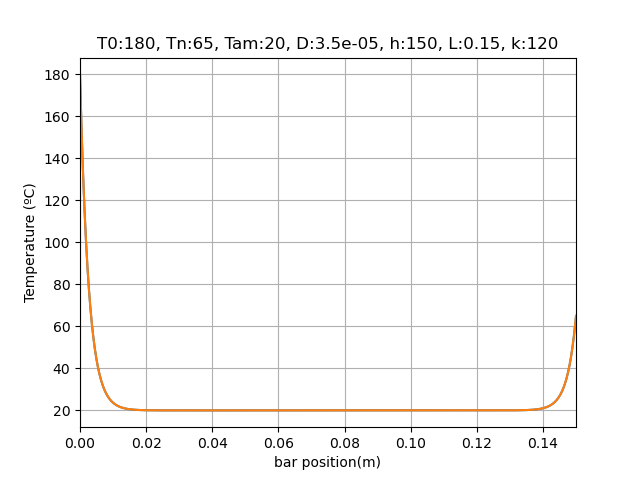
\includegraphics[scale=0.8]{figs/trd.png}
\end{figure}

\section{CONCLUSÃO}

Neste trabalho apresentamos o problema de transferência de calor em regime 
permanente. Também foi apresentado a formulação utilizanda para a solução, incluindo o sistema de equações, matrizes tridiagonais, ordem de erro, juntamente com simulações contendo as condições fornecidas pela tarefa bem como outras simulações contendo alterações em alguns componentes e discutimos que estas alterações significam em termos das características nos gráficos. 
% \section{REFERÊNCIAS:}

\end{document}
